%-------------------------
% Resume in Latex
% Author : Vladimir SIRGHI
%------------------------

% supports 10, 11, 12pt font sizes
% letterpaper = 8.5in x 11in
\documentclass[letterpaper,11pt]{article}

% set margins
\usepackage[
    left=0.5in,
    right=0.5in,
    top=0.4in,
    bottom=0.4in,
]{geometry}
\usepackage{latexsym}
\usepackage{titlesec}
\usepackage{marvosym}
\usepackage[usenames,dvipsnames]{color}
\usepackage{verbatim}
\usepackage{enumitem}
\usepackage[hidelinks]{hyperref}
\usepackage{fancyhdr}
\usepackage[english]{babel}
\usepackage{tabularx}
\usepackage{hyphenat}
\usepackage{fontawesome}
\usepackage{enumitem}
\input{glyphtounicode}
\usepackage{parskip}
\usepackage{graphicx}
\usepackage{etoolbox}  % for conditional logic
\usepackage{csquotes}


% is_long_version = true will render more detailed resume
\newtoggle{is_long_version} % Define the boolean variable
\settoggle{is_long_version}{false}

\pagestyle{fancy}

% clear all header and footer fields
\fancyhf{}
\fancyfoot{}
% remove lines between header/footer
\renewcommand{\headrulewidth}{0pt}
\renewcommand{\footrulewidth}{0pt}

\urlstyle{same}

% don't stretch text to fill the entire line
\raggedbottom
\raggedright
% remove horizontal padding from table cells
\setlength{\tabcolsep}{0in}

% Section heading formatting
\titleformat{\section}{
  \scshape\raggedright\large
}{}{0em}{}[\color{black}\titlerule]

% Ensure that generate pdf is machine readable/ATS parsable
\pdfgentounicode=1

%%% Set spacing %%%
% set vertical spacing between sections
\titlespacing*{\section}
{0pt} % left indent
{3pt} % spacing above
{3pt} % spacing below

\linespread{1.01}  % line spacing
\setlength{\parskip}{0pt} % paragraph spacing

% bullet list spacing
\setlist[itemize]{itemsep=0pt} % vertical spacing between bullets
\def\vspaceAfterBullets{3.5pt} % vertical spacing after bullet lists
\def\bulletIndent{20pt} % indent of bullet lists

% set bullet list symbol formatting
\setlist[itemize,1]{label=$\vcenter{\hbox{\tiny$\bullet$}}$}
\setlist[itemize,2]{label=$\vcenter{\hbox{\tiny$\bullet$}}$}
\setlist[itemize,3]{label=$\vcenter{\hbox{\tiny$\circ$}}$}

%-------------------------
% Custom commands

\newcommand{\bulletItem}[1]{
  \item\small{
    {#1}
  }
}

% company name -- location
\newcommand{\companyNameAndLocationHeading}[2]{
  \item
    \begin{tabular*}{1.0\textwidth}[b]{l@{\extracolsep{\fill}}r}
      \textbf{#1} & #2
    \end{tabular*}
}

% job title -- date
\newcommand{\titleAndDateHeading}[2]{
    \item
    \begin{tabular*}{1.0\textwidth}[b]{l@{\extracolsep{\fill}}r}
      {\bfseries\itshape\small #1} & \itshape\small #2
    \end{tabular*}
}

% project name -- date
\newcommand{\resumeProjectHeading}[2]{
    \item
    \begin{tabular*}{1.0\textwidth}[b]{l@{\extracolsep{\fill}}r}
      \small#1 & #2
    \end{tabular*}
}

\newcommand{\sectionListStart}{\begin{itemize}[leftmargin=0pt, label={}]}
\newcommand{\sectionListEnd}{\end{itemize}}

\newcommand{\outerBulletListStart}{\begin{itemize}[leftmargin=\bulletIndent]}
\newcommand{\outerBulletListEnd}{\end{itemize}\vspace{\vspaceAfterBullets}}


\newcommand{\innerBulletListStart}{\begin{itemize}[leftmargin=\bulletIndent]}
\newcommand{\innerBulletListEnd}{\end{itemize}}

% blue colored hyperlinks
\newcommand{\bref}[2]{\href{#1}{\color{blue}{#2}}}


%-------------------------------------------
%%%%%%  RESUME STARTS HERE  %%%%%%%%%%%
%
\begin{document}

%---------- HEADING ----------
% Header
\def\spaceAfterLogo{0.5pt}
 \begin{center}
   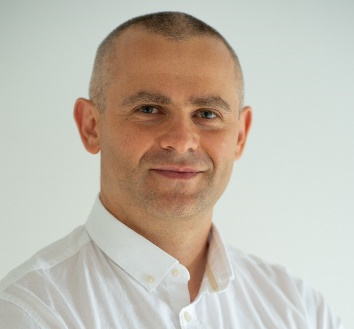
\includegraphics[width=3cm]{ressources/photo/cv_photo.jpg} \\[1em]
   \textbf{\LARGE Vladimir Sirghi} \\ \vspace{3pt}
   \small
   \faLinkedinSquare \hspace{\spaceAfterLogo} \href{https://www.linkedin.com/in/vladimir-sirghi/}{linkedin}
   $|$
   \faEnvelope \hspace{\spaceAfterLogo} \href{mailto:sirghivladimir@gmail.com}{sirghivladimir@gmail.com}
   $|$
   \faMobile \hspace{\spaceAfterLogo} \href{tel:+33638608085}{(+33) 638.60.80.85}
   $|$
   \faGithub \hspace{\spaceAfterLogo} \href{https://github.com/slalomeset}{github.com/slalomeset}
   $|$
   \faMapMarker \hspace{\spaceAfterLogo} \href{https://www.google.com/maps/place/Annecy}{Annecy, France}
 \end{center}

%----------- SUMMARY -----------
\iftoggle{is_long_version}
{
  \section{Personal Statement}
  \small Seasoned Robotics Control Engineer specializing in autonomous vehicles. Expert in control theory, trajectory optimization, and reinforcement learning. Passionate continuous learner, working on numerous side projects and taking online courses.
}{}

%----------- EXPERIENCE -----------

\section{Experience}
\sectionListStart

\companyNameAndLocationHeading {\bref{https://www.st.com/}{STMicroelectronics}}{Le Bourget-du-lac, Auvergne-Rhône-Alpes, France}
\titleAndDateHeading
{Embedded software engineer}{March 2022 \textbf{--} Present}
\outerBulletListStart
\bulletItem{Develop firmware for ARM Cortex-M targets and FPGAs SOC prototypes.}
\bulletItem{Lead and report on verification activities, ensuring thorough testing and validation.}
\bulletItem{Operate in an agile environment: address stories, tasks, tickets, sprints, issuing pull requests.}
\bulletItem{Provide support and guidance to external consultants throughout project execution.}
\bulletItem{Closely collaborate with digital design, architecture and test teams.}
\bulletItem{Document firmware design documentation.}
\bulletItem{Coding in C in automotive safety oriented projects.}
\bulletItem{Write cmake scripts for C/C++ project system build.}
\bulletItem{Use gcc and gdb for compilation and debugging.}
\bulletItem{Use and update low level drivers LL and HAL: hardware abstraction layers.}
\bulletItem{Bare metal coding.}
\bulletItem{Debug and optimize software in a cross-team environment.}
\bulletItem{Use git for versioning in a multiple nested repositories project environment.}
\bulletItem{Address, review pull-requests on github.}
\bulletItem{Develop in Windows, Linux, WSL, vscode windows to linux environments.}
\bulletItem{Write python and bash scripts to automate tasks and improve efficiency.}
\bulletItem{Make unit and integration tests.}
\bulletItem{Use Jenkins automated tasks, collaborate with the dev-ops to put in place new jobs.}
\bulletItem{Implemented mechanism allowing the user to extract reports on demand involving the ROS tool.}
\bulletItem{Developed firmware for power consumption profiling.}
\outerBulletListEnd
\vspace{1em} % Add space here
\companyNameAndLocationHeading
{\bref{https://atos.net/}{Atos}}{Grenoble, Auvergne-Rhône-Alpes, France}
\titleAndDateHeading
{Test engineer: cmos image sensors}{October 2020\textbf{--} February 2022}
\outerBulletListStart
\bulletItem{Developed Python testing scripts ensuring that the following safety mechanisms met safety requirements for the automotive industry:}
\innerBulletListStart
\bulletItem{mcu watchdog, stack monitoring, lockstep}
\bulletItem{firmware global variables protection,}
\bulletItem{at startup built in self tests bist}
\bulletItem{memory integrity, parity, bist,}
\bulletItem{crc program protection,}
\bulletItem{clock bist,}
\bulletItem{pll unlock detection,}
\bulletItem{asil diagnostic rows and columns,}
\bulletItem{otp memory crc,}
\bulletItem{supply monitoring blocks,}
\bulletItem{periodic voltage monitoring,}
\bulletItem{thermal monitoring,}
\bulletItem{periodic crack detection.}
\innerBulletListEnd

\bulletItem{Documented tests specifications and reported on test results.}
\bulletItem{Used git for code versioning, Jenkins for automation and integration}
\bulletItem{Wroked in agile environment.}
\outerBulletListEnd

\newpage

\companyNameAndLocationHeading
{\bref{https://www.st.com/}{STMicroelectronics}}{Grenoble, Auvergne-Rhône-Alpes, France}
\titleAndDateHeading
{Test engineer}{September 2018 \textbf{--} August 2020}
\outerBulletListStart
\bulletItem{Developed Python scripts for unitary, integration, and system tests on hardware and firmware components.}
\bulletItem{Documented tests requierements and reported on test results.}
\bulletItem{Used git for code versionning.}
\bulletItem{Solved and addressed tickets and issues on both hw and fw components.}
\outerBulletListEnd
\vspace{1em}

\companyNameAndLocationHeading
{\bref{https://www.defense.gouv.fr/terre}{French Army}}{Laudun - l'Ardoise, Occitanie, France}
\titleAndDateHeading
{Electro-mechanical technician and team lead}{September 2010 \textbf{--} August 2018}
\outerBulletListStart
\bulletItem{Managed military electrical networks, ensuring power supply and operational readiness.}
\bulletItem{Performed maintenance and troubleshooting on power plants and generator sets.}
\bulletItem{Designed and installed military electrical networks in external operations.}
\bulletItem{Led a team of military technicians, providing guidance, training, and support to ensure
quality work and team cohesion.}
\outerBulletListEnd
\sectionListEnd
\vspace{1em} % Add space here
%----------- EDUCATION -----------
\section{Education}
\sectionListStart
\companyNameAndLocationHeading
{\bref{https://scem-eset.univ-smb.fr/}{Savoie Mont Blanc University}}{Le Bourget-du-Lac, Auvergne-Rhône-Alpes, France}
\titleAndDateHeading
{\bref{https://github.com/slalomeset/diplomas/blob/main/master.pdf}{Masters in \enquote{Electronic of Embedded Systems and Telecommunications}}}{September 2018 \textbf{--} August 2020}
\outerBulletListStart
\bulletItem{Telecommunications electronics}
\bulletItem{Fast signal electronics and EMC}
\bulletItem{Microwave circuits}
\bulletItem{Signal processing}
\bulletItem{DSP signal processing processors}
\bulletItem{C programming for embedded systems}
\bulletItem{Radiocoms \& Wireless LAN}
\bulletItem{FPGAs and reconfigurable processors}
\bulletItem{IP networks and Internet of Things}
\bulletItem{Programmable systems-on-chips}
\bulletItem{High speed transmission}
\bulletItem{Error detection and correction}
\bulletItem{Computer architecture}
\bulletItem{Principles of radiocomunication}
\bulletItem{Antennas}
\bulletItem{Communication bus systems and networks}
\bulletItem{Integrated radio frequency components}
\bulletItem{Linux kernels for embedded systems}
\bulletItem{Real time on microprocessor target}
\bulletItem{Digital circuit technology and design}
\bulletItem{Applications of embedded systems in telecoms}
\bulletItem{Advanced Integrated Components}
\bulletItem{Energy production and management for systems}
\outerBulletListEnd
\vspace{1em} % Add space here

\companyNameAndLocationHeading
{\bref{https://sup-fc.univ-fcomte.fr/informatique}{University of Franche-Comté}}{Bourgogne-Franche-Comté, France}
\titleAndDateHeading
{Bachelor in \enquote{Computer Science}}{September 2020 \textbf{--} August 2021}
\outerBulletListStart
\bulletItem{Data base}
\bulletItem{Algorithms and Basics of Programming}
\bulletItem{English}
\bulletItem{Analysis and modeling of information systems}
\bulletItem{Formal methods}
\bulletItem{Computer architecture}
\bulletItem{Systems and Networks}
\bulletItem{Language theory}
\bulletItem{Program specification and proof}
\bulletItem{Web languages}
\bulletItem{Advanced programming}
\outerBulletListEnd
\newpage % Jump to new page

\companyNameAndLocationHeading
{\bref{https://www.univ-tlse3.fr/decouvrir-nos-diplomes/licence-parcours-eea-fondamental-eea-f}{Toulouse 3 University \enquote{Paul Sabatier}}}{Toulouse, Occitanie, France}
\titleAndDateHeading
{\bref{https://github.com/slalomeset/diplomas/blob/main/bachelor.pdf}{Bachelor in \enquote{Electronics, Electrical Engineering and Automation.}}}{September 2016 \textbf{--} August 2018}
\outerBulletListStart
\bulletItem{Operating systems for control computers.}
\bulletItem{Computer process linking.}
\bulletItem{ADC/DAC converters.}
\bulletItem{C language: pointers and sequential files.}
\bulletItem{Interpolation, adjustment, and optimization.}
\bulletItem{Laplace, Fourier, Z-transform, and sampling.}
\bulletItem{MATLAB language and matrix calculations.}
\bulletItem{Propagation of a signal in free and guided space.}
\bulletItem{Transfer functions.}
\bulletItem{Quadrupoles.}
\bulletItem{Resolution of linear and non-linear systems.}
\bulletItem{Linear programming.}
\bulletItem{Analog diode circuits, static and switching transistors.}
\bulletItem{Amplifiers, field-effect transistors, and counter-reaction.}
\bulletItem{Insulating materials, magnetic circuits, three-phase distribution networks, and single-phase transformers.}
\bulletItem{Synchronous machines: alternators and motors; asynchronous motors.}
\bulletItem{DC/DC converters, switching power supplies, and single-phase inverters; speed variation of a direct current machine.}
\bulletItem{Temporal and frequency modeling of elementary dynamic systems (mechanical, electro-mechanical, etc.).}
\bulletItem{Performance analysis of a controlled system and summary of an analog control strategy.}
\outerBulletListEnd
\vspace{1em}

\companyNameAndLocationHeading
{\bref{https://www.cned.fr/}{CNED \enquote{Centre National d'Enseignement à Distance}}}{Avignon, Provence-Alpes-Côte d’Azur, France}
\titleAndDateHeading
{\bref{https://github.com/slalomeset/diplomas/blob/main/bts.pdf}{BTEC HND in \enquote{Electrical Engineering and Electronics }}}{September 2014 \textbf{--} August 2016}
\outerBulletListStart
\bulletItem{Mathematics}
\bulletItem{Applied Sciences}
\bulletItem{Construction}
\bulletItem{Electrical Engineering}
\bulletItem{English}
\bulletItem{General Culture and Expression}
\outerBulletListEnd
\vspace{1em} % Add space here

\companyNameAndLocationHeading
{\bref{https://www.armyacademy.ro/engleza/fmm.php}{\enquote{Nicolae Balcescu} Land Forces Academy }}{Sibiu, Romania }
\titleAndDateHeading
{\bref{https://github.com/slalomeset/diplomas/blob/main/military_academy.pdf}{ Bachelor's Degree in Management of Military Organizations }}{September 2002 \textbf{--} August 2006}
\outerBulletListStart
\bulletItem{Faculty of Military Management has the mission to form, at undergraduate and postgraduate level, officers for arms/military specialties of the Land Forces and also military and civilian specialists for other beneficiaries from the national defence system, public order and national security. The mission is in total accordance with the Institutional Strategy of “Nicolae Balcescu” Land Forces Academy and aims at creating general and specific professional competencies for the arms/military specialties: Artillery, Engineering, Defense CBRN, Transportation, Intendance, Finances and Accounting, Communications and Informatics.}
\outerBulletListEnd

\sectionListEnd
\vspace{1em} % Add space here


\section{Languages}
\sectionListStart
\bulletItem{\textbf{English:}{ Professional}}
\bulletItem{\textbf{French:}{ Native}}
\bulletItem{\textbf{Romanian:}{ Native}}
\sectionListEnd
\vspace{1em} % Add space here

%----------- SKILLS -----------

\section{Skills \& Interests}
\sectionListStart
\bulletItem{\textbf{Languages:}{ C, python, bash, MATLAB}}
\vspace{\vspaceAfterBullets}
\bulletItem{\textbf{Technologies \& tools:}{ Ubuntu/Linux, Git, CMake, \LaTeX, ROS, OpenOcd, Cortex M, Jenkins, gcc/gdb, jlink/stlink}}
\vspace{\vspaceAfterBullets}
\bulletItem{\textbf{Protocols:}{ i2c, spi, uart, jtag, swd, can}}
\vspace{\vspaceAfterBullets}
\bulletItem{\textbf{Continued Education:}}
\outerBulletListStart
\bulletItem{\bref{https://www.udemy.com/course/mastering-rtos-hands-on-with-freertos-arduino-and-stm32fx/}{Mastering RTOS: Hands on FreeRTOS and STM32Fx with Debugging}}
\bulletItem{\bref{https://www.udemy.com/course/bash-mastery/?kw=Bash+Mastery\%3A+The+Complete+Guide+to+Bash+Shell+Scriptin&src=sac}{Bash Mastery: The Complete Guide to Bash Shell Scripting}}
\bulletItem{\bref{https://www.udemy.com/course/embedded-system-programming-on-arm-cortex-m3m4/}{Embedded Systems Programming on ARM Cortex-M3 M4 Processor}}
\bulletItem{\bref{https://www.udemy.com/course/microcontroller-programming-stm32-timers-pwm-can-bus-protocol/}{Mastering Microcontroller: Timers, PWM, CAN, Low Power (MCU2)}}
\bulletItem{\bref{https://www.udemy.com/course/embedded-linux-step-by-step-using-beaglebone/}{Embedded Linux Step by Step Using Beaglebone Black}}
\bulletItem{\bref{https://www.udemy.com/course/complete-python-bootcamp/}{The Complete Python Bootcamp From Zero to Hero in Python}}
\bulletItem{\bref{https://www.udemy.com/course/git-complete}{Git Complete: The definitive, step-by-step guide to Git}}
\bulletItem{\bref{https://www.udemy.com/course/mastering-microcontroller-with-peripheral-driver-development/?kw=Mastering+Microcontroller+and+Embedded+Driver+Development&src=sac}{Mastering Microcontroller and Embedded Driver Development}}
\bulletItem{\bref{https://www.udemy.com/course/stm32f4-arm-cortex-mx-custom-bootloader-development/?couponCode=25BBPMXINACTIVE}{STM32Fx Microcontroller Custom Bootloader Development}}
\bulletItem{\bref{https://www.udemy.com/course/microcontroller-embedded-c-programming/?kw=Microcontroller+Embedded+C+Programming\%3A+absolute+beginners&src=sac}{Microcontroller Embedded C Programming: Absolute Beginners}}


\outerBulletListEnd
\vspace{\vspaceAfterBullets}
\bulletItem{\textbf{Interests:}{ family activities \& education, music, cross-training}}
\sectionListEnd
\vspace{1em} % Add space here

%----------- PROJECTS -----------
\section{Projects}
\sectionListStart

\resumeProjectHeading
{\textbf{Moving Cube Image } }

\outerBulletListStart
\bulletItem{C application running on a stm32fx target reading X, Y, Z values from the joystick's accelerometer}
\bulletItem{Based on X, Y, Z values dynamically display the position of the cube on the screen}
\outerBulletListEnd

\resumeProjectHeading
{\textbf{Convolutional encoding machine \& viterbi decoder } }

\outerBulletListStart
\bulletItem{ Python application running convolutional encoder on data}
\bulletItem{ GUI (developed in QT) allowing the user to enter textual message in data field \& explicetly corrupt some bits}
\bulletItem{ transmitting corrupted payload to the stm32fx via uart}
\bulletItem{ stm32fx running a viterbi decoder and printing the fixed message on a lcd}
\outerBulletListEnd

\resumeProjectHeading
{\textbf{PID PWM motor control } }

\outerBulletListStart
\bulletItem{ C code embedded into stm32fx ram memory running application}
\bulletItem{ application reading temperature from a temperature sensor }
\bulletItem{ based on temperature value outputing a PWM signal}
\bulletItem{ increasing the PWM duty cycle with the temperature increase}
\bulletItem{ a cooler motor controlled through PWM energy }
\outerBulletListEnd

\resumeProjectHeading
{\textbf{Maximum Power Point Tracking MPPT Solar Panel Controller} }

\outerBulletListStart
\bulletItem{ C application running on PIC16F877A microcontroller }
\bulletItem{ reading voltage and current from the solar panel}
\bulletItem{ calculating the maximum power point using the Perturb \& Observe algorithm}
\bulletItem{ adjusting the duty cycle of a DC-DC converter to optimize power output}
\bulletItem{ implementing a sun tracking system to follow the sun's position for maximum illumination}
\bulletItem{ charging a battery \& powering a water pump}
\outerBulletListEnd
\sectionListEnd

%-------------------------------------------
\end{document}
